\documentclass{standalone}
\usepackage{tikz}
\usetikzlibrary{patterns, positioning}
\usepackage[sfdefault]{ClearSans} %% option 'sfdefault' activates Clear Sans as the default text font
\usepackage[T1]{fontenc}

\begin{document}
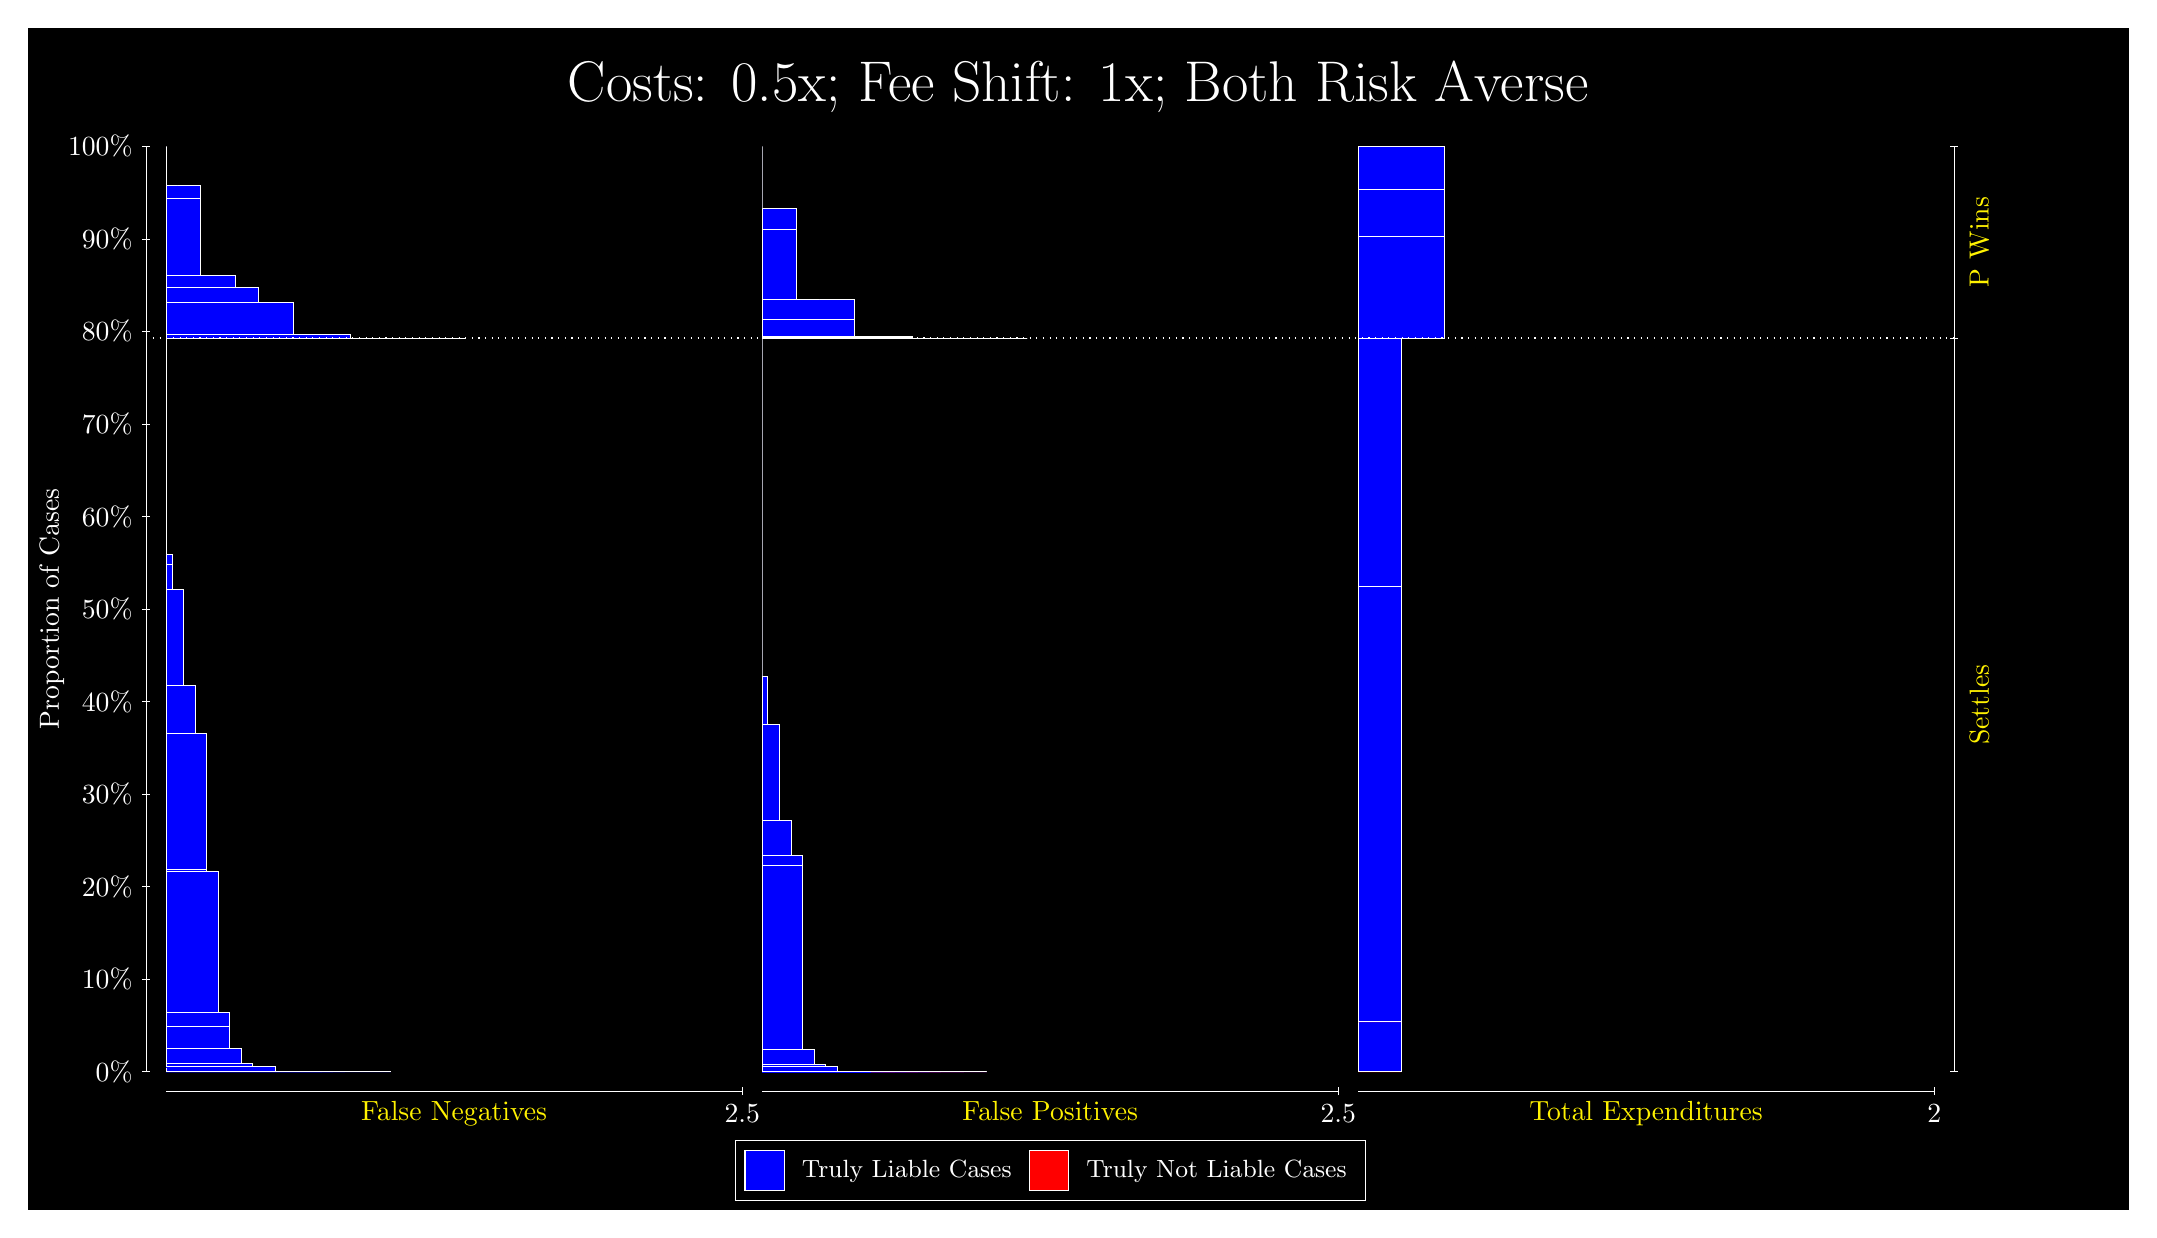
\begin{tikzpicture}
\draw[fill=black] (0,0) rectangle (26.667,15);
\draw[text=white] (0,13.5) rectangle (26.667,15) node[midway] {\huge Costs: 0.5x; Fee Shift: 1x; Both Risk Averse};
\draw[white, very thin] (1.5,1.75) -- (1.5,13.5);
\node[rotate=90, text=white, anchor=center] at (0.3, 7.625) {Proportion of Cases};
\draw[white, very thin] (1.45,1.75) -- (1.55,1.75);
\node[text=white, anchor=east] at (1.45, 1.75) {0\%};
\draw[white, very thin] (1.45,2.925) -- (1.55,2.925);
\node[text=white, anchor=east] at (1.45, 2.925) {10\%};
\draw[white, very thin] (1.45,4.1) -- (1.55,4.1);
\node[text=white, anchor=east] at (1.45, 4.1) {20\%};
\draw[white, very thin] (1.45,5.275) -- (1.55,5.275);
\node[text=white, anchor=east] at (1.45, 5.275) {30\%};
\draw[white, very thin] (1.45,6.45) -- (1.55,6.45);
\node[text=white, anchor=east] at (1.45, 6.45) {40\%};
\draw[white, very thin] (1.45,7.625) -- (1.55,7.625);
\node[text=white, anchor=east] at (1.45, 7.625) {50\%};
\draw[white, very thin] (1.45,8.8) -- (1.55,8.8);
\node[text=white, anchor=east] at (1.45, 8.8) {60\%};
\draw[white, very thin] (1.45,9.975) -- (1.55,9.975);
\node[text=white, anchor=east] at (1.45, 9.975) {70\%};
\draw[white, very thin] (1.45,11.15) -- (1.55,11.15);
\node[text=white, anchor=east] at (1.45, 11.15) {80\%};
\draw[white, very thin] (1.45,12.325) -- (1.55,12.325);
\node[text=white, anchor=east] at (1.45, 12.325) {90\%};
\draw[white, very thin] (1.45,13.5) -- (1.55,13.5);
\node[text=white, anchor=east] at (1.45, 13.5) {100\%};

\draw[white, very thin] (24.457,1.75) -- (24.457,13.5);
\draw[white, very thin] (24.407,1.75) -- (24.507,1.75);
\node[anchor=west] at (24.407, 1.75) {};
\draw[white, very thin] (24.407,11.066) -- (24.507,11.066);
\node[anchor=west] at (24.407, 11.066) {};
\draw[white, very thin] (24.407,13.5) -- (24.507,13.5);
\node[anchor=west] at (24.407, 13.5) {};

\draw[white, very thin, fill=blue] (1.75,1.75) rectangle (4.6044,1.75);
\draw[white, very thin, fill=blue] (1.75,1.75) rectangle (4.0188,1.75);
\draw[white, very thin, fill=blue] (1.75,1.75) rectangle (3.8725,1.75);
\draw[white, very thin, fill=blue] (1.75,1.75) rectangle (3.7261,1.75);
\draw[white, very thin, fill=blue] (1.75,1.75) rectangle (3.4333,1.7504);
\draw[white, very thin, fill=blue] (1.75,1.7504) rectangle (3.287,1.7519);
\draw[white, very thin, fill=blue] (1.75,1.7519) rectangle (3.1406,1.8115);
\draw[white, very thin, fill=blue] (1.75,1.8115) rectangle (2.9942,1.8125);
\draw[white, very thin, fill=blue] (1.75,1.8125) rectangle (2.8478,1.8567);
\draw[white, very thin, fill=blue] (1.75,1.8567) rectangle (2.7015,2.042);
\draw[white, very thin, fill=blue] (1.75,2.042) rectangle (2.5551,2.3259);
\draw[white, very thin, fill=blue] (1.75,2.3259) rectangle (2.5551,2.5041);
\draw[white, very thin, fill=blue] (1.75,2.5041) rectangle (2.4087,4.2933);
\draw[white, very thin, fill=blue] (1.75,4.2933) rectangle (2.2623,4.3226);
\draw[white, very thin, fill=blue] (1.75,4.3226) rectangle (2.2623,6.0481);
\draw[white, very thin, fill=blue] (1.75,6.0481) rectangle (2.1159,6.6556);
\draw[white, very thin, fill=blue] (1.75,6.6556) rectangle (1.9696,7.8775);
\draw[white, very thin, fill=blue] (1.75,7.8775) rectangle (1.8232,8.1902);
\draw[white, very thin, fill=blue] (1.75,8.1902) rectangle (1.8232,8.3167);
\draw[white, very thin, fill=red] (1.75,8.3167) rectangle (1.75,8.3167);
\draw[white, very thin, fill=blue] (1.75,8.3167) rectangle (1.75,11.066);
\draw[white, very thin, fill=blue] (1.75,11.066) rectangle (5.5558,11.066);
\draw[white, very thin, fill=blue] (1.75,11.066) rectangle (4.8239,11.067);
\draw[white, very thin, fill=blue] (1.75,11.067) rectangle (4.3848,11.067);
\draw[white, very thin, fill=blue] (1.75,11.067) rectangle (4.092,11.117);
\draw[white, very thin, fill=blue] (1.75,11.117) rectangle (3.6529,11.117);
\draw[white, very thin, fill=blue] (1.75,11.117) rectangle (3.3602,11.518);
\draw[white, very thin, fill=blue] (1.75,11.518) rectangle (2.921,11.715);
\draw[white, very thin, fill=blue] (1.75,11.715) rectangle (2.6283,11.858);
\draw[white, very thin, fill=blue] (1.75,11.858) rectangle (2.1891,12.845);
\draw[white, very thin, fill=blue] (1.75,12.845) rectangle (2.1891,13.004);
\draw[white, very thin, fill=blue] (1.75,13.004) rectangle (1.8964,13.004);
\draw[white, very thin, fill=red] (1.75,13.004) rectangle (1.75,13.004);
\draw[white, very thin, fill=blue] (1.75,13.004) rectangle (1.75,13.5);
\draw[white, very thin, fill=red] (9.3189,1.75) rectangle (12.173,1.75);
\draw[white, very thin, fill=blue] (9.3189,1.75) rectangle (12.173,1.75);
\draw[white, very thin, fill=red] (9.3189,1.75) rectangle (11.88,1.75);
\draw[white, very thin, fill=blue] (9.3189,1.75) rectangle (11.88,1.75);
\draw[white, very thin, fill=red] (9.3189,1.75) rectangle (11.588,1.75);
\draw[white, very thin, fill=blue] (9.3189,1.75) rectangle (11.588,1.75);
\draw[white, very thin, fill=blue] (9.3189,1.75) rectangle (11.441,1.75);
\draw[white, very thin, fill=red] (9.3189,1.75) rectangle (11.295,1.75);
\draw[white, very thin, fill=blue] (9.3189,1.75) rectangle (11.295,1.75);
\draw[white, very thin, fill=blue] (9.3189,1.75) rectangle (11.149,1.75);
\draw[white, very thin, fill=red] (9.3189,1.75) rectangle (11.002,1.75);
\draw[white, very thin, fill=blue] (9.3189,1.75) rectangle (11.002,1.75);
\draw[white, very thin, fill=blue] (9.3189,1.75) rectangle (10.856,1.75);
\draw[white, very thin, fill=red] (9.3189,1.75) rectangle (10.709,1.75);
\draw[white, very thin, fill=blue] (9.3189,1.75) rectangle (10.709,1.7503);
\draw[white, very thin, fill=blue] (9.3189,1.7503) rectangle (10.563,1.7505);
\draw[white, very thin, fill=red] (9.3189,1.7505) rectangle (10.417,1.7505);
\draw[white, very thin, fill=blue] (9.3189,1.7505) rectangle (10.417,1.7545);
\draw[white, very thin, fill=blue] (9.3189,1.7545) rectangle (10.27,1.8131);
\draw[white, very thin, fill=blue] (9.3189,1.8131) rectangle (10.124,1.8443);
\draw[white, very thin, fill=blue] (9.3189,1.8443) rectangle (9.9776,2.0305);
\draw[white, very thin, fill=red] (9.3189,2.0305) rectangle (9.8312,2.0305);
\draw[white, very thin, fill=blue] (9.3189,2.0305) rectangle (9.8312,4.373);
\draw[white, very thin, fill=blue] (9.3189,4.373) rectangle (9.8312,4.4991);
\draw[white, very thin, fill=blue] (9.3189,4.4991) rectangle (9.6848,4.9384);
\draw[white, very thin, fill=blue] (9.3189,4.9384) rectangle (9.5384,6.1603);
\draw[white, very thin, fill=blue] (9.3189,6.1603) rectangle (9.3921,6.7678);
\draw[white, very thin, fill=blue] (9.3189,6.7678) rectangle (9.3189,11.066);
\draw[white, very thin, fill=red] (9.3189,11.066) rectangle (12.686,11.066);
\draw[white, very thin, fill=blue] (9.3189,11.066) rectangle (12.686,11.066);
\draw[white, very thin, fill=red] (9.3189,11.066) rectangle (11.954,11.066);
\draw[white, very thin, fill=blue] (9.3189,11.066) rectangle (11.954,11.066);
\draw[white, very thin, fill=blue] (9.3189,11.066) rectangle (11.954,11.066);
\draw[white, very thin, fill=red] (9.3189,11.066) rectangle (11.222,11.066);
\draw[white, very thin, fill=blue] (9.3189,11.066) rectangle (11.222,11.073);
\draw[white, very thin, fill=blue] (9.3189,11.073) rectangle (11.222,11.087);
\draw[white, very thin, fill=red] (9.3189,11.087) rectangle (10.783,11.087);
\draw[white, very thin, fill=blue] (9.3189,11.087) rectangle (10.783,11.087);
\draw[white, very thin, fill=red] (9.3189,11.087) rectangle (10.49,11.087);
\draw[white, very thin, fill=blue] (9.3189,11.087) rectangle (10.49,11.299);
\draw[white, very thin, fill=blue] (9.3189,11.299) rectangle (10.49,11.562);
\draw[white, very thin, fill=red] (9.3189,11.562) rectangle (10.051,11.562);
\draw[white, very thin, fill=blue] (9.3189,11.562) rectangle (10.051,11.562);
\draw[white, very thin, fill=blue] (9.3189,11.562) rectangle (9.758,12.442);
\draw[white, very thin, fill=blue] (9.3189,12.442) rectangle (9.758,12.708);
\draw[white, very thin, fill=red] (9.3189,12.708) rectangle (9.3189,12.708);
\draw[white, very thin, fill=blue] (9.3189,12.708) rectangle (9.3189,13.5);
\draw[white, very thin, fill=red] (16.888,1.75) rectangle (17.437,1.75);
\draw[white, very thin, fill=blue] (16.888,1.75) rectangle (17.437,2.3837);
\draw[white, very thin, fill=red] (16.888,2.3837) rectangle (17.437,2.3837);
\draw[white, very thin, fill=blue] (16.888,2.3837) rectangle (17.437,7.9141);
\draw[white, very thin, fill=red] (16.888,7.9141) rectangle (17.437,7.9141);
\draw[white, very thin, fill=blue] (16.888,7.9141) rectangle (17.437,11.066);
\draw[white, very thin, fill=red] (16.888,11.066) rectangle (17.986,11.066);
\draw[white, very thin, fill=blue] (16.888,11.066) rectangle (17.986,12.362);
\draw[white, very thin, fill=red] (16.888,12.362) rectangle (17.986,12.362);
\draw[white, very thin, fill=blue] (16.888,12.362) rectangle (17.986,12.958);
\draw[white, very thin, fill=red] (16.888,12.958) rectangle (17.986,12.958);
\draw[white, very thin, fill=blue] (16.888,12.958) rectangle (17.986,13.5);
\draw[white, dotted] (1.5,11.066) -- (24.457,11.066);
\draw[white, very thin] (1.75,1.5) -- (9.0689,1.5);
\node[text=yellow, anchor=north] at (5.4094, 1.5) {False Negatives};
\draw[white, very thin] (9.0689,1.45) -- (9.0689,1.55);
\node[text=white, anchor=north] at (9.0689, 1.45) {2.5};

\draw[white, very thin] (9.3189,1.5) -- (16.638,1.5);
\node[text=yellow, anchor=north] at (12.978, 1.5) {False Positives};
\draw[white, very thin] (16.638,1.45) -- (16.638,1.55);
\node[text=white, anchor=north] at (16.638, 1.45) {2.5};

\draw[white, very thin] (16.888,1.5) -- (24.207,1.5);
\node[text=yellow, anchor=north] at (20.547, 1.5) {Total Expenditures};
\draw[white, very thin] (24.207,1.45) -- (24.207,1.55);
\node[text=white, anchor=north] at (24.207, 1.45) {2};

\node[text=yellow, centered, rotate=90] at (24.777, 6.4079) {Settles};
\node[text=yellow, centered, rotate=90] at (24.777, 12.283) {P Wins};

\draw (12.978300999999998,1.5) node[draw=none] (baseCoordinate) {};
\begin{scope}[align=center]
        \matrix[scale=0.5, draw=white, below=0.5cm of baseCoordinate, nodes={draw}, column sep=0.1cm]{
            \node[rectangle, draw, minimum width=0.5cm, minimum height=0.5cm, fill=blue] {}; &
            \node[draw=none, font=\small, text=white] (B) {Truly Liable Cases}; &
            \node[rectangle, draw, minimum width=0.5cm, minimum height=0.5cm, fill=red] {}; &
            \node[draw=none, font=\small, text=white] (B) {Truly Not Liable Cases}; \\
            };
\end{scope}

\end{tikzpicture}
\end{document}